\documentclass[]{report}
\usepackage{float}
\usepackage{parskip}
\usepackage[]{fbb}
\usepackage[top=45mm, bottom=45mm, left=25mm, right=25mm]{geometry}
\usepackage{listings}
\usepackage{tikz}
\usetikzlibrary{positioning, arrows.meta, decorations.markings, decorations.pathreplacing}
\usepackage{amsmath}
\usetikzlibrary{positioning, shapes.geometric, arrows}
\usepackage{mathrsfs}
\usepackage{booktabs}

\renewcommand{\arraystretch}{2}

\title{\textbf{AISE3010: Assignment 2}}
\date{\textit{February 26, 2024}}
\author{Arnav Goyal - 251244778 \\ Malak Al-Hanafi - 251142157}

\begin{document}
\maketitle
	
\section*{The Submission}
Our submission is a \texttt{.zip} file that extracts to the following directories:
\begin{itemize}
	\item \texttt{aise3010\_assignment2\_q1.py} - referred to as the 'q1' script
	\item \texttt{aise3010\_assignment2\_q2.py} - referred to as the 'q2' script
	\item \texttt{models.py}
	\item \texttt{checkpoints/...}
	\item \texttt{data/...}
\end{itemize}
The \texttt{models.py} script holds the architecture for the models used in the Script, specifically \texttt{'Net2'} for part 1 and \texttt{'MidwayClassifer'} for part 2.

The question 1 script (\texttt{aise3010\_assignment2\_q1.py}) trains and tests the entire custom CNN architecture, it allows the user to train/test from scratch or train/test from a 'train checkpoint' stored at \texttt{checkpoints/Net2.pth}. The question 2 script (\texttt{aise3010\_assignment2\_q2.py}) extracts a feature midway through the convolutional part of the \texttt{Net2} CNN model, and trains a MLP classifier using these features as data. You can also train/test from scratch or train/test from a 'train checkpoint' stored at \texttt{checkpoints/MidwayClassifier.pth}. The \texttt{data} folder stores the CIFAR-10 dataset, which we used in this assignment.

\section*{Testing/Grading The Submission}
To grade/use the submission you have two choices, we recommend saving some time by using the train checkpoints we provided:
\begin{itemize}
	\item Use the train checkpoints - See Option 1
	\item Train both networks from scratch - See Option 2
\end{itemize}
The following sections will talk about the models/workings of the script.

\subsection*{Option 1: Using The Train Checkpoints}
This is the easy way to test this submission, essentaially we have stored the state dictionaries from our pretrained models as \texttt{.pth} files in the \texttt{checkpoints} folder so you don't have to train them again! \textit{Note:} These were trained with a batch size of 32, 20 epochs, 0.001 learning rate, and 0.9 momentum.

To proceed with this option, first open the q1 script, and enter \texttt{1} into the console to start from a checkpoint. The script will then load the checkpoint \texttt{Net2.pth} before prompting you again, at this point enter a \texttt{1} into the console to test from this loaded checkpoint. The console will then print out the test accuracy of the entire designed network. This completes question 1.
\textit{Note}: our checkpoint provides an accuracy of about 61.82\%

For question 2, open up the q2 script and enter a \texttt{1} into the console to load from the provided checkpoint at \texttt{checkpoints/MidwayClassifier.pth}. This will load our pre-trained MLP classifier trained on the midway extracted features from the model in question 1. After this, you will be prompted for input again, at this point enter a \texttt{1} to test from this checkpoint. This first extracts features midway from the q1 model, and feeds them into the MLP classifier, and prints the accuracy of this classifier.
This completes question 2. \textit{Note:} Our checkpoint provides a testing accuracy of about 50.99\%

\textit{Note:} Feel free to play around while running the scripts, to further train from checkpoints, or see Option 2 to train and save new checkpoints from scratch - everything \textit{should} work fine$\ldots$

\subsection*{Option 2: Training From Scratch}
This is the long way, regardless, open up script q1 and enter a \texttt{2} into the console when prompted, this lets the script know you arent using the checkpoints, and are opting to train for 20 epochs instead. At this point the training will begin and after about 108 years it will finish, you will then be shown a training curve, and upon closing it the program will ask if you would like to overwrite the current checkpoint, I would suggest entering a \texttt{1} to save these weights (this will overwrite the ones we provided, but you can always replace them with ours from the original submission's files). At this point testing will begin and will display accuracy once it is complete. This completes question 1.

For question 2, run script q2 and enter \texttt{2} to train the midway feature classifier from scratch. This will start the training process, and displays the training curve after training. After closing the plot window, you will be prompted again, enter a \texttt{1} to save these weights and overwrite ours, similar to how you did in q1. The testing process will then begin and it will display accuracy at the end.

\section*{The Models}

We use two models: \texttt{'Net2'} is our designed CNN for question 1, and \texttt{'MidwayClassifier'} is the classifier we trained to predict classes based on the extracted features midway through the forward pass of the \texttt{Net2} model's convolutional layers. Diagrams are shown below for ease of understanding

\vspace{1em}
\begin{center} \centering \textbf{Model 1:} The Custom Designed CNN - \texttt{'Net2'} for Question 1 \\
	\textit{\small Note that each orange conv block represents a convolution layer + relu + max pooling. Note that each green fc block features a fully-connected layer + relu activation} \\
	\vspace{1em}
	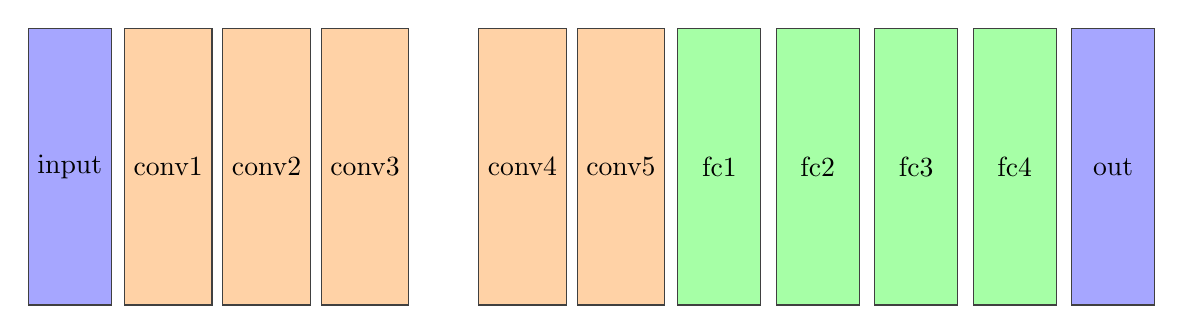
\begin{tikzpicture}[draw=darkgray, node distance=1.25cm]
	%diagram
	\node[draw, rectangle, minimum height=10em, minimum width=3em, fill=blue!35] (input) {input};
	\node[draw, rectangle, minimum height=10em, minimum width=3em, fill=orange!35, right of=input] (conv1) {conv1};
	\node[draw, rectangle, minimum height=10em, minimum width=3em, fill=orange!35, right of=conv1] (conv2) {conv2};
	\node[draw, rectangle, minimum height=10em, minimum width=3em, fill=orange!35, right of=conv2] (conv3) {conv3};
	\node[draw, rectangle, minimum height=10em, minimum width=3em, fill=orange!35, right of=conv3, node distance=2cm] (conv4) {conv4};
	\node[draw, rectangle, minimum height=10em, minimum width=3em, fill=orange!35, right of=conv4] (conv5) {conv5};
	\node[draw, rectangle, minimum height=10em, minimum width=3em, fill=green!35, right of=conv5] (fc1) {fc1};
	\node[draw, rectangle, minimum height=10em, minimum width=3em, fill=green!35, right of=fc1] (fc2) {fc2};
	\node[draw, rectangle, minimum height=10em, minimum width=3em, fill=green!35, right of=fc2] (fc3) {fc3};
	\node[draw, rectangle, minimum height=10em, minimum width=3em, fill=green!35, right of=fc3] (fc4) {fc4};
	\node[draw, rectangle, minimum height=10em, minimum width=3em, fill=blue!35, right of=fc4] (out) {out};
\end{tikzpicture} \end{center}
\newpage
\begin{center} \centering \textbf{Model 2:} The Midway Classifier - \texttt{'MidwayClassifier'} for Question 2 \\
	\textit{\small This is an Single-Layer Network designed to train/predict classes of extracted features from an input feature taken between conv3 and conv4 of the \texttt{Net2} CNN (shown above). Note that each green fc block features a fully-connected layer + relu activation} \\
	\vspace{1em}
	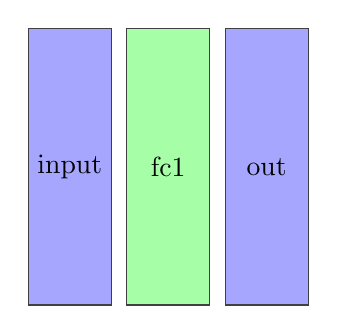
\begin{tikzpicture}[draw=darkgray, node distance=1.25cm]
		%diagram
		\node[draw, rectangle, minimum height=10em, minimum width=3em, fill=blue!35] (input) {input};
		\node[draw, rectangle, minimum height=10em, minimum width=3em, fill=green!35, right of=input] (fc1) {fc1};
		\node[draw, rectangle, minimum height=10em, minimum width=3em, fill=blue!35, right of=fc1] (out) {out};
\end{tikzpicture} \end{center}
\vspace{2em}
The detailed layer parameters of both models are contained within the \texttt{models.py} script and will not be re-explained here for sake of brevity (this report is so long already).

The important part is the the q1 script trains \textbf{Model 1} with CIFAR-10 and tests this model as well, and that the q2 script uses CIFAR-10 on the trained Model 1 to get the midway features from between layers conv3 and conv4, and then feeds this extracted feature into \textbf{Model 2} for training and/or testing purposes.

\section*{Analysis \& Improvement}
The results (training accuracy) we get make sense due to the differences in both models. Model 1 is vastly more complex than Model 2, and hence it achieves more accuracy on this complex image dataset (CIFAR-10). We could also train for some more time, as it seems both models haven't plateau'd in terms of the training curve as of yet. These curves are attached below. Realistically we should also take care to not overfit to our training dataset. This is esepcially more likely with Model 2 due to its small size. Regardless, training for more epochs does seem to somewhat increase the test accuracy, so we could do that or use a different (maybe better?) architecture in Model 1 to increase this accuracy as well. \newpage

\begin{center}
	\centering
	\textbf{Plot 1:} Training Curve from Question 1 Script \\
	\includegraphics[scale=0.55]{Q1_Curve.png}
\end{center}

\begin{center}
	\centering
	\textbf{Plot 2:} Training Curve from Question 2 Script \\
	\includegraphics[scale=0.55]{Q2_Curve.png}
\end{center}

\end{document}